\documentclass[11pt]{article}
\usepackage{enumitem}
\usepackage{amssymb}
\usepackage{amsmath}
\usepackage{graphicx}
\usepackage{float}

\graphicspath{{images/}}

\begin{document}
\title{MAT1830 --- Assignment 7}
\author{Dylan Pinn --- 24160547}
\maketitle

\section*{Question 1}

Let $R$ be the relation on $\mathbb{Z} \times \mathbb{Z}$ defined by $(w, x)R(y,
z)$ if any only if $w + x \leq y + z$.

\noindent
Let $S$ be the relation on $\mathbb{Z} \times \mathbb{Z}$ defined by $(w, x)S(y,
z)$ if and only if $w \leq y$ and $x \leq z$

\begin{enumerate}[label= (\alph*)]
  \item Is $R$ antisymmetric?

  Yes. Because the relation is defined across integers, if we make $w + x$ some
    integer $a$ and $y + z$ soem integer $b$. Then we can show that for any $a,b
    \in \mathbb{Z}$ we have that $a \leq b$ or $b \leq a \Rightarrow a = b$.

  \item Is $S$ antisymmetric?

    No. Because we can show that for $(1, 4)\not S(2, 2)$ and $(2,2) \not
    S(1,4)$

\end{enumerate}
\break{}

\section*{Question 2}

You know the following facts about a relation $T$:

\begin{itemize}
  \item $T$ is defined on the set $\{a, b, c, d, e \}$,
  \item $aTc, bTc, cTd, eTb$ and $e\not{T}a$,
  \item $T$ is a partial order relation.
\end{itemize}

Draw a Hasse diagram for every possible relation that $T$ could be and, for
each, write down whether it is a total order relation.

\begin{center}
    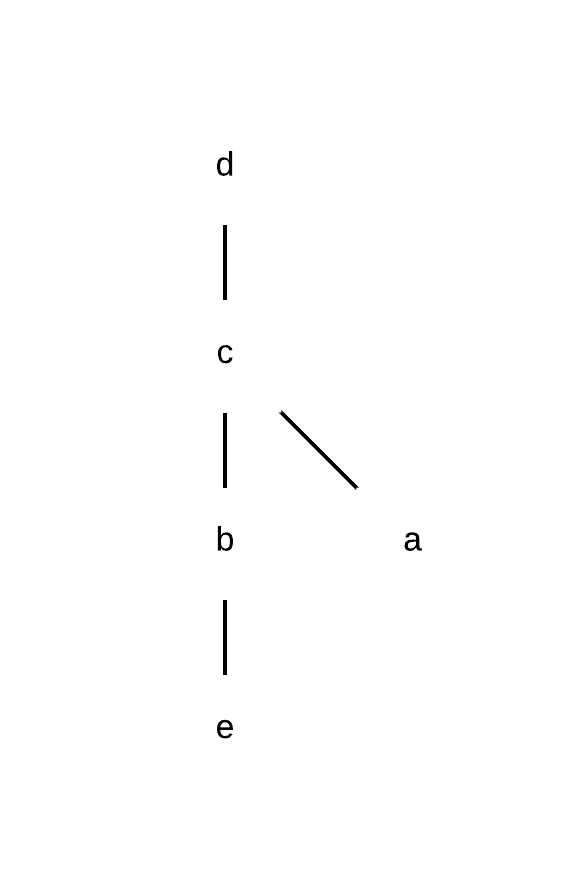
\includegraphics{A7}
\end{center}

No, not total order relation.

\break{}
\section*{Question 3}

Find expressions for each of the following

\begin{enumerate}[label= (\alph*)]
  \item The number of strings of 7 lower case letters (a-z) that do not contain
    any letter twice or more.

    As we need to do unordered selections without repetition it will be:
  \[
    = \binom{n}{r} \\
    = \binom{26}{7}
  \]

  \item The number of binary strings of length 50 that contain at most three 1s.

    As we want to get all of these that contain at most three it will be:

    \[
      =\binom{50}{0} + \binom{50}{1} + \binom{50}{2} + \binom{50}{3}
    \]

  \item The number of ternary strings of length 10 (strings of 0s, 1s and 2s)
    containing exactly one 1 and exactly four 2s.

    We want to find the strings such that 1222200000. As order is not important
    it will be and we don't want repetition. It is:

    \[
      =\binom{10}{5}
    \]

\end{enumerate}

\break{}
\section*{Question 4}

A small school with 14 students has a basketball team with 5 players, a chess
team with 4 players, a netball team with 7 players, and a soccer team with 11
players.

\begin{itemize}
  \item Each student is on at least one of these teams and no student is on all
    four teams.
  \item Only one student, Hawa, is on three of the teams; she plays chess,
    netball and soccer.
  \item There is exactly 1 student who plays basketball and chess.
  \item There is exactly 1 student who plays basketball and netball.
  \item Hawa is the only student who plays chess and netball.
  \item There are exactly 3 students (including Hawa) who play chess and soccer.
  \item There are exactly 5 students (including Hawa) who play netball and
    soccer.
\end{itemize}

How many students play basketball and soccer?

\begin{align*}
  |B \cup C \cup N \cup S| &= |B| + |C| + |N| + |S| \\
  &- |B \cap C| - |B \cap N| - |B \cap S| - |C \cap N| - |C \cap S| - |N \cap
  S| \\
  &+|B \cap C \cap N| + |B \cap C \cap S| + |B \cap N \cap S| + |C \cap N \cap
  S| \\
  &- |B \cap C \cap N \cap S| \\
  14 &= 5 + 4 + 7 + 11 - 1 - 1 - x - 1 - 3 - 5 + 1 + 0 + 0 + 0 + 0 - 0 \\
  14 &= 17 - x \\
  -3 &= -x \\
  x &= 3
\end{align*}

Therefore there are three students how play soccer and basketball.

\end{document}
